%%%%%%%%%%%%%%%%%%%%%%%%%%%%%%%%%%%%%%%%%%%%%%%%%%%%%%%%%%%%%%%%%%%%%%%%%%%%%%
\chapter{Synthesis of a Framework for Learning and Social HRI} \label{chap:behavemodel}

\begin{framed}
	\textbf{Key points:}
	
	\begin{itemize}
	\item Previous chapters have made many comparisons between different robot social behaviours and their impact on child \gls{learning}. This chapter draws these behaviours together through the common metric of \gls{nonverbalimm}.
	\item A further experimental condition is devised and data is gathered using a human tutor for the prime numbers task to provide a contextual baseline for the robot behaviours.
	\item Nonverbal immediacy does not fully explain the differences in child \gls{learning} between robot conditions.
	\item A framework for child \gls{learning} as a product of social cues and cue congruency is put forwards to provide an explanation for the data here and to make predictions for future work.
	\end{itemize}
\end{framed}

The work presented in this chapter is under review in \cite{kennedy2016impact}.

\newpage
The primary tenet of the thesis exists in the relationship between robot social behaviour and child \gls{learning}. This section will seek to discuss this relationship in detail, drawing on the experimental work conducted throughout this document, alongside additional data collected here. First, the methodology of the additional experimental condition will be outlined. This will be followed by a critical discussion of \gls{nonverbalimm} in relation to the thesis and the research questions identified in Section \ref{sec:intro-thesis}.

%%%%%%%%%%%%%%%%%%%%%%%%%%%%%%%%%%%%%%%%%%%%%%%%%%%%%%%%%%%%%%%%%%%%%%%%%%%%%%
\section{Human Prime Tutoring} \label{sec:disc-humanprimes}
One question that often arises, particularly from non-academic audiences, is how robots compare to human tutors. The aim of research into robot tutors is rarely to replace human teaching, but to supplement it, so such a comparison is not typically part of experimental hypotheses. Given the link between robot social behaviour and \gls{learning} (Chapter~\ref{chap:nviexperiment}), human behaviour is often used to derive behaviour for robots to provide an upper benchmark of social behaviour that robots can aim for in tutoring. The literature from other fields suggests that human tutoring also provides an upper benchmark in terms of \gls{learning} gains. \cite{vanlehn2011relative} finds that human tutoring produces an effect size of \textit{d}=0.79, while \acrshort{its} produces an effect of about \textit{d}=0.76. However, this comparison has not been verified in \acrshort{hri}. 

\cite{serholt2014comparing} found no significant difference between the performance of children who had been tutored by a humanoid robot compared to a human, but the robot speech was controlled using a Wizard-of-Oz method, introducing additional variability between conditions. The present section reports on data collected from running an additional condition using the prime tutoring task, in which the lesson content was delivered by a human. The purpose of this additional data collection is to provide a benchmark for child \gls{learning} when a human delivers exactly the same content, but using their natural social cues. The findings will be considered in later sections in combination with robot conditions from this thesis.

\subsection{Methodology}
This study employs one condition: a human tutor teaching the prime numbers task to provide a benchmark comparison for the robot conditions used in previous chapters. The study employs the same methodology as seen in Chapters~\ref{chap:socasoc} and~\ref{chap:nviexperiment}. Children aged 8 and 9 engage in a dyadic interaction in their school with a tutor who guides them through a method for prime number identification. The children's \gls{learning} is measured through a pre-test and a post-test consisting of 12 numbers which need to be categorised as `prime' or `not prime' (6 per category). Prior to the interaction, children have not learnt about prime numbers, but the technique relies on their ability to divide by 2, 3, 5 and 7, so this is also tested. The tutor provides hints to help with the division, as well as a lesson about how to identify prime numbers using the Sieve of Eratosthenes technique. Two tests for prime number identification are used in a cross-testing strategy to control for exposure to the tests.

The human was given a word-by-word script to match the lesson content of the robot from Chapter~\ref{chap:nviexperiment}, but was not constrained in terms of social behaviour. Due to the script providing precise lesson content (and the study focus on social behaviour and embodiment differences) an expert tutor was not required. 11 children took part in the study (age \textit{M}=8.8, \textit{SD}=0.4), with interactions lasting for \textit{M}=13m10 (\textit{SD}=3m39).

\subsection{Results}
The pre- and post-test scores are paired values on a continuous measure, distributions did not significantly deviate from normality (Kolmogorov-Smirnov test; $\textit{p}>.05$). As such, a paired samples \textit{t}-test is used for analysis. Children improve significantly; the post-test score (\textit{M}=7.6, 95\% CI [5.5,9.8]) is significantly higher than the pre-test score (\textit{M}=5.2, 95\% CI [3.7,6.7]); \textit{t}(10)=2.425, \textit{p}=.036 (Figure \ref{fig:ch10_humangraph}). The effect size seen here is \textit{d}=0.89, which is not so dissimilar to that seen in \cite{vanlehn2011relative}, where human tutoring averages \textit{d}=0.79. As such, this provides some reassurance of the validity of the tutoring undertaken. Although it should be noted that the effect sizes in \citet{vanlehn2011relative} compare to a no tutoring control, which is not done here since the nature of the task makes \gls{learning} unlikely without tutoring.

\begin{figure}[t]
    \centering
    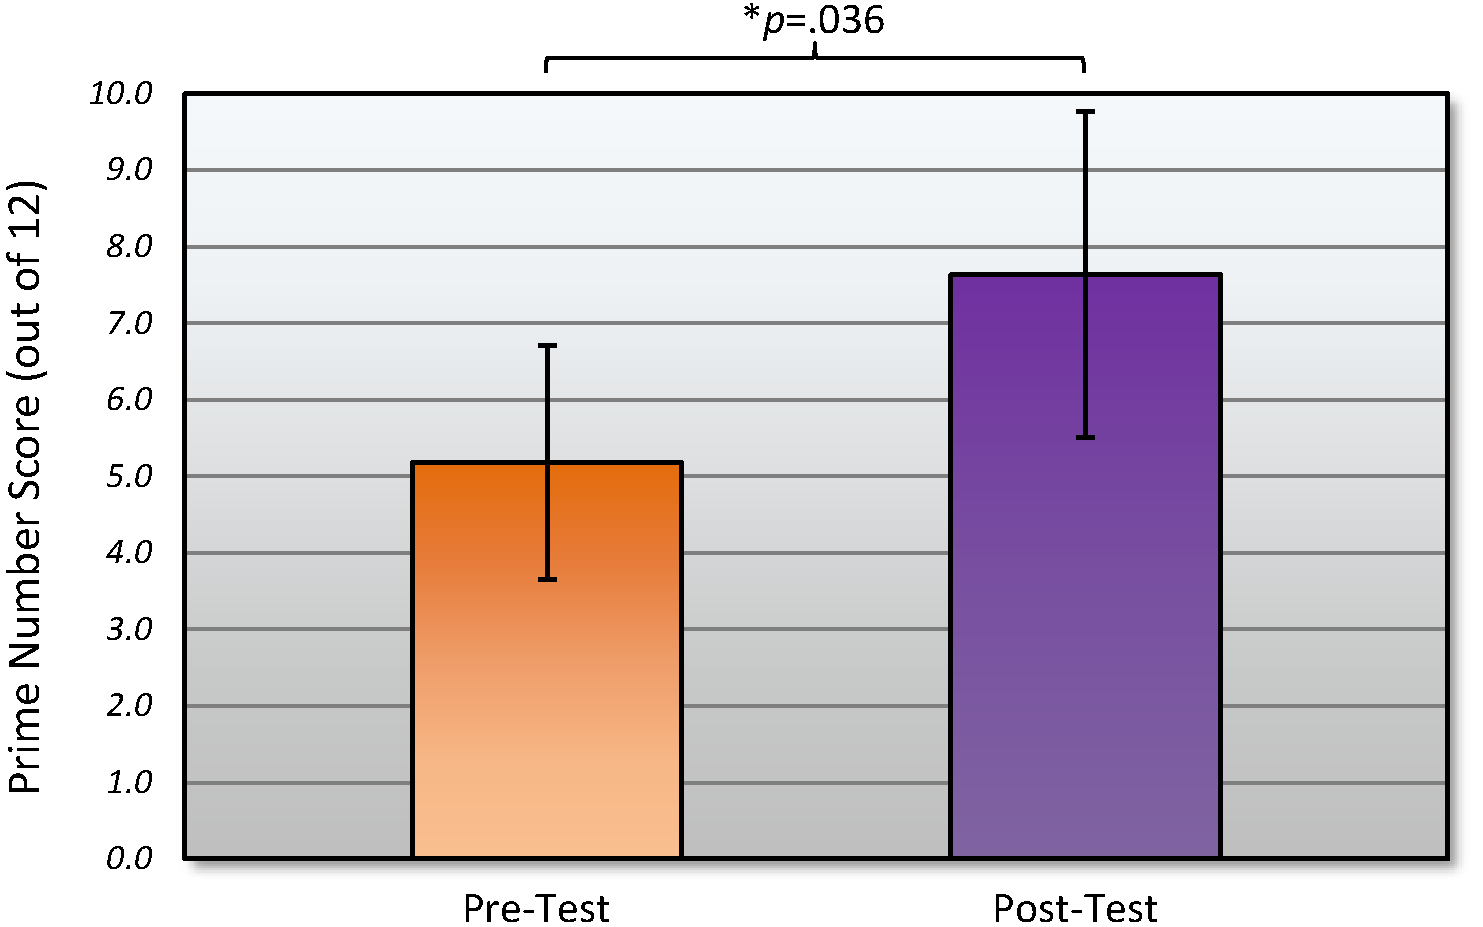
\includegraphics[width=0.75\textwidth]{images/ch10_HumanGraph.pdf}
    \caption{Pre-test and post-test scores for prime number learning of children when tutored by a human. The children improve significantly from the pre-test to the post-test. \textit{Error bars} show 95\% Confidence Interval.}
    \label{fig:ch10_humangraph}
\end{figure}

It is also worth noting that the mean was lowered by one instance where the child had clearly learnt the technique, but confused the categories, and so scored 0 on the post-test (i.e., 100\%, but incorrect). The child asked for clarification, but as this help would not have been available when the content was delivered by the robot (as in Chapter \ref{chap:nviexperiment}), it was not given by the human at the time.

The specific human used in the tutoring task may have had an impact on the results. The social behaviour was not constrained, which meant that the human could take advantage of some social cues that the robot could not, and could subsequently be more socially adaptive (for example, in mutual gaze) than a robot, which may account for some of the \gls{learning} differences. A non-expert human was used due to the tightly specified learning content, but an expert tutor may have used different social behaviour, potentially leading to more \gls{learning}. Overall, the children rated the human behaviour \gls{nonverbalimm} on average \textit{M}=54.4 (95\% CI [52.9,55.9]) using the \acrshort{cniq} from Appendix \ref{app:cniq}. The findings here will subsequently be further explored in the context of the robot conditions previously used in the prime tutoring task.

%%%%%%%%%%%%%%%%%%%%%%%%%%%%%%%%%%%%%%%%%%%%%%%%%%%%%%%%%%%%%%%%%%%%%%%%%%%%%%
\section{Nonverbal Immediacy and Learning}\label{sec:chap9-nonvlearn}
Five different conditions have been used in the prime number learning task\footnote{This section refers only to the physically embodied conditions, not the `no lesson', or `no robot' control conditions presented in Chapter \ref{chap:socasoc}.}. For three of these conditions, \gls{nonverbalimm} scores were collected directly from the children, and for all five, adult \gls{nonverbalimm} scores are available. Taking \gls{nonverbalimm} as a characterisation of robot social behaviour \citep{kennedy2015less}, these results can be used to support the central thesis: a robot with tailored social behaviour will improve child \gls{learning}. The graphs in Figures~\ref{fig:ch10_nvilearngraph_adult} and~\ref{fig:ch10_nvilearngraph_child} show a clear trend towards greater \gls{nonverbalimm} leading to increased child \gls{learning}. This is further supported through the strong positive correlation between the \gls{learning} effect sizes (Cohen's \textit{d}) and the \gls{nonverbalimm} scores (as judged by adults); \textit{r}(3)=0.70. This provides additional support for the thesis on top of that presented in individual experimental chapters.

\begin{figure}[t]
    \centering
    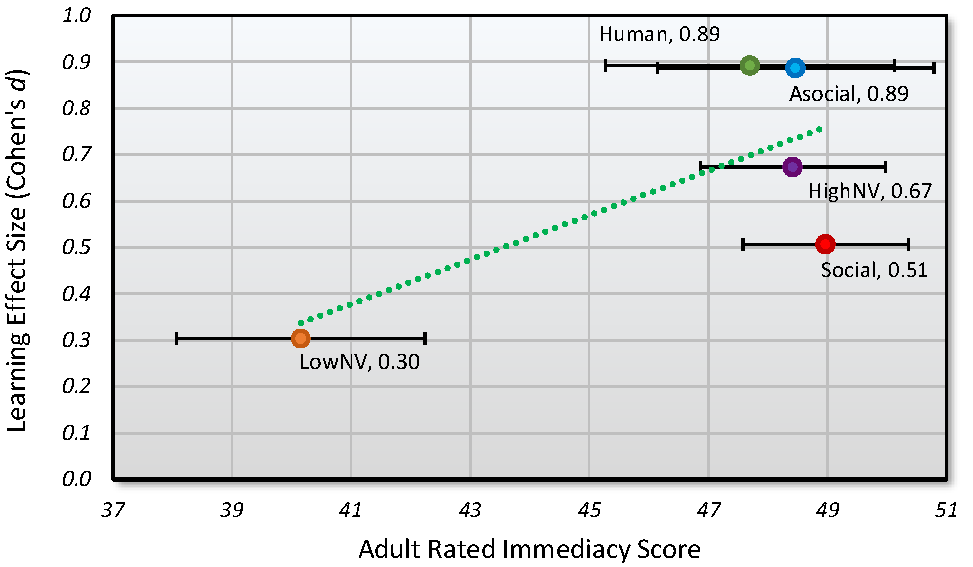
\includegraphics[width=0.75\textwidth]{images/ch10_adultnvilearn.pdf}
    \caption{Nonverbal immediacy scores as judged by adults and learning effect sizes for the prime number task. The dotted green line indicates a trend towards greater \gls{nonverbalimm} of the tutor leading to increased \gls{learning}. \textit{Error bars} show 95\% Confidence Interval.}
    \label{fig:ch10_nvilearngraph_adult}
\end{figure}

\begin{figure}[t]
    \centering
    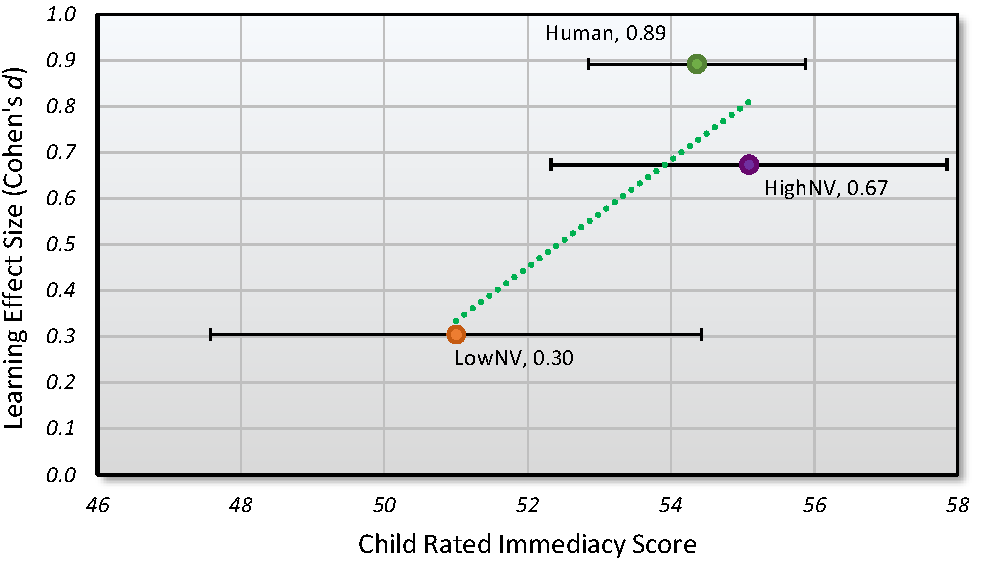
\includegraphics[width=0.75\textwidth]{images/ch10_childnvilearn.pdf}
    \caption{Nonverbal immediacy scores as judged by the children in the interaction and \gls{learning} effect sizes for the prime number task. The dotted green line indicates a trend towards greater perceived \gls{nonverbalimm} of the tutor leading to increased learning. \textit{Error bars} show 95\% Confidence Interval.}
    \label{fig:ch10_nvilearngraph_child}
\end{figure}

Much of this thesis considers social behaviour as characterised through immediacy. It is recognised that immediacy is not a complete measure of social behaviour; indeed it has several shortcomings as such (detailed shortly). Nevertheless, immediacy provides a characterisation of the social behaviour through the overt cues displayed by the robot. Using these overt cues allows more meaningful responses from children than other surveys of child perception typically do \citep{kennedy2015characterise}, and Chapter \ref{chap:validation} showed that \gls{nonverbalimm} allows transfer from existing \acrshort{hhi} literature to \acrshort{chri}. These findings, combined with the clear relevance of social cues to social behaviour, support the use of immediacy as a proxy for social behaviour. 

However, \gls{nonverbalimm} does not account for all of the differences in \gls{learning}. Three of the conditions have near identical \acrshort{nvi} scores as judged by adults, but quite varied \gls{learning} results (high \acrshort{nvi} robot: \textit{M}=48.4 \acrshort{nvi} score/\textit{d}=0.67 pre-post test improvement, asocial robot: \acrshort{nvi} \textit{M}=48.5/\textit{d}=0.89, social robot: \acrshort{nvi} \textit{M}=49.0/\textit{d}=0.51). This partially reflects the slightly mixed picture of immediacy that the \acrshort{hhi} literature presents, for example, the disagreement as to whether \acrshort{nvi} has a linear \citep{christensen1998linear} or curvilinear \citep{comstock1995food} relationship with \gls{learning}. Nonetheless, there are further factors that may be introduced by the use of a robot that may have had an influence on the results. Nonverbal immediacy only considers overt observed social behaviours, so by design does not cover all possible aspects of effective social behaviour for tutoring. Whilst this seems to be enough in \acrshort{hhi} \citep{witt2004meta}, it may not be for \acrshort{hri}. Several possible explanations as to why this \gls{learning} variation is present will now be discussed. From this, a possible model (suggested to be more accurate) of the relationship between social behaviour and \gls{learning} is proposed. Such a model may be useful in describing (and testing) the relationship between social behaviour and child \gls{learning} for future research.

\subsection{Timing of Social Cues}
The quantity of social cues used in both the social robot and asocial robot conditions is exactly the same, however the timing is varied. Timing is not considered as part of the \acrshort{nvi} metric - the scale measures whether cues have, or have not, been used, rather than whether their timing was appropriate. The cues used in the asocial robot condition were intentionally placed at inappropriate times (for example, waving part-way through the introduction, instead of when saying hello). This is not factored into the \acrshort{nvi} measure, but could impact the \gls{learning} \citep{nussbaum1992effective}.

The timing of social cues in the human condition may also explain why the \gls{learning} in this condition was higher than the others. The robot conditions are all either non-adaptive, or minimally adaptive (the social robot condition will seek mutual gaze using the Kinect sensor) in the timing of cues. However, the human is presumably adaptive in both the number of social cues used and the timing of these cues. Again, this would not be directly revealed by the \acrshort{nvi} metric, but could account for some of the \gls{learning} difference. Indeed, the \acrshort{nvi} metric comes from \acrshort{hhi} studies and has been validated in such environments. In \acrshort{hhi}, there is a reasonable assumption that the timing of social cues will be appropriate, and so it may not be necessary to include it as part of a behavioural metric for \acrshort{hhi}. However, when applied to social robotics, the assumption of appropriate timing no longer applies and so to fully account for \gls{learning} differences in \acrshort{hri}, timing may need more explicit incorporation into characterisations of social behaviour.

\subsection{Adaptation of Social Cues}
Personalised adaptation of social cues has previously been suggested to be an important factor in \acrshort{hri} \citep{dautenhahn2004robots, tapus2008user}. Many researchers have sought to adapt elements of the teaching strategy of a robot to humans \citep{leyzberg2014personalizing, gordon2015bayesian, westlund2015interplay}, however this strand of research appears to be less concerned with robot social cues and more with optimal teaching approaches in \acrshort{hri} contexts. Adaptation of robot social cues -- focusing on the social behaviour/interaction itself, rather than higher-level teaching strategy -- remains relatively underexplored in educational contexts.

Both \cite{szafir2012pay} and \cite{brown2013applying} have used timing of social cues in response to models of human engagement in order to try and `re-engage' learners in an interaction. Differing degrees of success were achieved in the two studies, but the potential of robot social behaviour for positively influencing \gls{learning} in educational scenarios is clearly demonstrated. However, these models could be pushed further, with adaptive social behaviour throughout the interaction rather than just in response to specific events such as detected dis-engagement. Such an example would be multimodal behavioural alignment, as discussed in \cite{baxter2014pervasive}, or adaptive personalisation as implemented in \cite{coninx2015towards}. Adaptation of social cues is, like timing of social cues, not explicitly included in the \acrshort{nvi} measure, possibly because it can be assumed in \acrshort{hhi}.

\subsection{Relative Importance of Social Cues}
One substantial difference between the robot conditions and the human condition is the possibility of using facial expressions. The robotic platform used for the studies was the Aldebaran NAO. This platform has limited ability to generate facial expressions as none of the elements of the face can move, only the eye colour can be changed. On the other hand, the human has a rich set of facial expressions to draw upon.

Whilst the overall \acrshort{nvi} scores for the asocial, social and human conditions are tightly bunched, the make-up of the scores is not. For example, the robot scores (asocial and social combined) are higher for gesturing, averaging \textit{M}=4.3 (95\% CI [4.1,4.5]) out of 5 for the \gls{nonverbalimm} question about gesturing (the robot uses its hands and arms to gesture while talking to you), compared to \textit{M}=3.1 (95\% CI [2.7,3.5]) for the human. However, the human is perceived to smile more (\textit{M}=2.5, 95\% CI [2.1,2.8]) than the robot (\textit{M}=1.8, 95\% CI [1.5,2.0]). Through principle component analysis, \cite{wilson2007immediacy} found that different elements of nonverbal behaviour do not contribute equally to either the \gls{nonverbalimm} construct, nor to instructor effectiveness. Facial expressions (specifically smiles) have a large impact on both the \gls{nonverbalimm} construct and on instructor effectiveness, whereas gestures do not have such a large effect (although still a meaningful contribution; smiles: .54, gestures: .30 component contribution from \citealp{wilson2007immediacy}).

In the \acrshort{nvi} metric, all social cues are given equal weighting. However, this may not always be the most appropriate method for combining the cues given the evidence which suggests that some cues may contribute more than others to various outcomes \citep{mccroskey1996nonverbal, wilson2007immediacy}. This could be a further explanation as to why several of the conditions under examination here have near identical overall \acrshort{nvi} scores, but very different \gls{learning} outcomes. Considering each of the sub-scales (i.e., social cues) independently would also not account for \gls{learning}, as they should be judged in context \citep{zaki2013cue}. Nonverbal immediacy is designed to cope with characterising social behaviour across a multitude of contexts, and to weight the importance of cues in a metric could become problematic. When robots are used, due to their different morphological features and capabilities, substantial empirical evidence would need to be gathered for each platform to generate accurate weightings. These would then only apply in the context involving that platform, thus reducing much of the versatility offered by relatively context-free metrics like immediacy.

\subsection{Novelty of Character and Behaviour}
The novelty of both the character (i.e., robot or human) and of the behaviour itself could have had an impact on the \gls{learning} results found in the study. Novelty is highlighted as a potential issue in both of the chapters in which the robot conditions were presented for the first time (\ref{chap:socasoc} and \ref{chap:nviexperiment}), as well as in other experiments conducted in the field \citep{kanda2004interactive, sung2009robots}. More long-term studies need to be conducted in order reduce and account for novelty effects.

The novelty of the robot behaviour could override the differences between the conditions and subsequently influence the \gls{learning} of the child. In the social robot condition here, novel behaviour (such as new gestures) was often introduced when providing lessons to the child. Between humans, this would likely result in a positive effect \citep{goldin2001explaining}, but when done by a robot, the novelty of the behaviour may counter-act the intended positive effect.

There may also be a difference in the novelty effect for the children seeing the robot when compared to the human. Although the human is not one that they are familiar with, they are still `just' a human, whereas the robot is likely to be more exciting and novel as child interaction with robots is more limited than with humans. The additional novelty of the robot could have been a distraction from the \gls{learning}, explaining why the \gls{learning} in the human condition is higher. Alternatively, the manipulations to the robot's immediacy behaviour may not be interpreted in the same way as they would be in a typical classroom, which could influence the outcome of higher immediacy behaviours; this has previously been suggested to be a factor in human-human studies of immediacy \citep{christensen1998linear}.

Finally, the novelty may have impacted the \acrshort{nvi} scores themselves. It is possible that observers (be they children or adults) score immediacy on a relative scale. It is reasonable to suggest that the immediacy of the characters is judged not as a standalone piece of behaviour, but in the context of an observer's prior experience, or expectations for what that character may be capable of. Clear expectations will likely exist for human behaviour, but not for robot behaviour, which may lead to an over-estimation of robot immediacy. This would impact on the ability of considering the human and robots on the same \gls{nonverbalimm} scale and drawing correlations with \gls{learning}, and cannot be ruled out as a factor in the results.

\subsection{(In)congruency of Social Cues}
As previously discussed, the robot is limited in the social cues that it can produce (for example, it cannot produce facial expressions). This meant that the conditions all manipulated the available robot social cues, but if social cues are interpreted as a single percept by the human (as suggested by the literature \citealp{zaki2013cue}), then this could lead to complications.

In the case of the social robot, many social cues are used to try and maximise the `sociality' of the robot. This means that there is a lot of gaze from the robot to the child and the robot uses a lot of gestures. However, it still cannot produce facial expressions. This incongruency between the social cues could produce an adverse effect in terms of perception on the part of the child and subsequently diminish the \gls{learning} outcome. There are clear parallels here with the concept of the Uncanny Valley \citep{mori2012uncanny}, with models for the Uncanny Valley based on category boundaries in perception indicating issues arising from these mismatches \citep{moore2012bayesian}.

The expectation the child has for the robot social behaviour is suggested to be of great importance \citep{kennedy2015less}. If their expectations are formed early on through high quantities of gaze and gestures, then there would be a discrepancy when facial expressions do not match this expectation. Again, this expectation discrepancy may lead to adverse effects on \gls{learning} outcomes, as in the case of perceptual issues due to cue incongruence. These issues may become exacerbated as the overall level of sociality of behaviour of the robot increases as any incongruences then become more pronounced. As stated in \cite{richmond1987nonverbal}, higher immediacy generally leads to more communication, which can create misperceptions (of liking, or expected behaviour).

As robot social behaviour consists of a multitude of social cues, and the congruence between these cues may play an important role in the overall perception of the behaviour, the need to explore the congruency between cues arises. To achieve this, the \gls{nonverbalimm} scale is returned to, as whilst this is calculated on the basis of a combination of many social cues, the cues are rated on an individual basis. The \gls{nonverbalimm} scale has been rigorously validated \citep{mccroskey1996nonverbal,richmond2003development}, and it is known that it provides a reliable metric for the immediacy construct which it attempts to measure in humans (Cronbach's Alpha is typically between 0.70 and 0.85; \citealp{mccroskey1996nonverbal}). Chapter \ref{chap:validation} of this document provided a validation of the scale adapted by the author for use with robots (adapted scales are shown in Appendices \ref{app:rniq} and \ref{app:cniq}). When used with adult respondents reporting on robot behaviour, it was found that this adapted scale had a comparably high internal consistency rating ($\alpha=.79$) to the original scale used with humans.

Typically, internal consistency measures of a scale, like Cronbach's alpha, would be used to evaluate the ability of a scale to measure a unidimensional construct. With the assumption (evidenced through the high internal consistency measures from experimental work) that the \acrshort{nvi} scale is indeed unidimensional, it becomes feasible to consider that if a robot behaviour is rated and the internal consistency value is low, this is not a reflection on the scale (which is known to be reliable), but instead on the behaviour. Through the nature of the robot's capabilities there are several \acrshort{nvi} scale items which are known to be impaired. For example, the robot cannot produce facial expressions. If all of the other social cues that form the scale are manipulated such that they reflect `high' \acrshort{nvi}, then the lack of facial expressions will cause the internal consistency measure to drop. Based on this logic, it is suggested that internal consistency measures could be used as an indicator of the incongruence between social cues within the immediacy scale. The greater the internal consistency, the more congruent the social cues could be, but a lower internal consistency indicates larger variability between scale items, and thus possibly larger incongruency between the cues.

Guttman's $\lambda _{6}$ (or G6) for each condition has been calculated\footnote{Cronbach's alpha tends to be the de facto standard for evaluating internal consistency and reliability, however its use as such a measure has been called into question \citep{revelle2009coefficients} -- including by its own creator \citep{cronbach2004my}. Instead G6 is used which considers the amount of variance in each item that can be accounted for by the linear regression of all other items (the squared multiple correlation; \citealp{guttman1945basis}). Like Cronbach's alpha, G6 normally ranges from 0 to 1, with values closer to 1 indicating higher internal consistency reliability. This provides a lower bound for item communality, becoming a better estimate with increased numbers of items. This would appear to provide a logical (but likely imperfect) indicator for the congruency of cues as required here.}, revealing that indeed there are differences in how congruent the cues could be considered to be (Table \ref{tab:guttman}; Figure \ref{fig:ch10-guttmangraph}). The behavioural conditions used here are restricted in such a way that a lower reliability would be expected (as several cues of the scale are not utilised) for some conditions. Indeed, these values fall in line with predictions that could be made based on the social behaviour in each of the conditions. The human reliability score provides a ``sanity check'' as it is assumed that human behaviour would have a certain degree of internal consistency between social cues, which is reflected by it having the highest value. Additionally, the low \acrshort{nvi} robot condition has intentionally low \acrshort{nvi} behaviour, so the lack of smiling or touching (high \acrshort{nvi} behaviours) does not cause incongruency (signified by a lower G6 score), whereas the high \acrshort{nvi} robot condition has intentionally high \acrshort{nvi} behaviour where possible on the robot, so the lack of smiling and touching causes greater overall incongruency, resulting in a considerably lower G6 score.

\begin{table}[t!]
	\centering
	\renewcommand{\arraystretch}{1.2} 
	\begin{tabular}{@{}lcc@{}}
	\toprule
	\textbf{Condition} & \begin{tabular}[x]{@{}c@{}}\textbf{Learning Effect Size}\\ \textbf{(Cohen's \textit{d})}\end{tabular} & \textbf{Guttman's Lambda 6 (G6)} \\ \midrule
	Asocial robot (Chapter \ref{chap:socasoc})  				& 0.89                 & 0.84                             \\
	Social robot (Chapter \ref{chap:socasoc})   					& 0.51                 & 0.83                             \\
	High NVI robot (Chapter \ref{chap:nviexperiment}) 	& 0.67                 & 0.69                             \\
	Low NVI robot (Chapter \ref{chap:nviexperiment})  	& 0.30                 & 0.78                             \\
	Human (Chapter \ref{chap:behavemodel})          			& 0.89                 & 0.87                             \\ \bottomrule
\end{tabular}
\caption{Guttman's G6 and \gls{learning} effect size by condition. G6 is used as an indicator of social cue congruency, with a higher value indicating greater congruency between cues.}
\label{tab:guttman}
\end{table}

\begin{figure}[t]
    \centering
    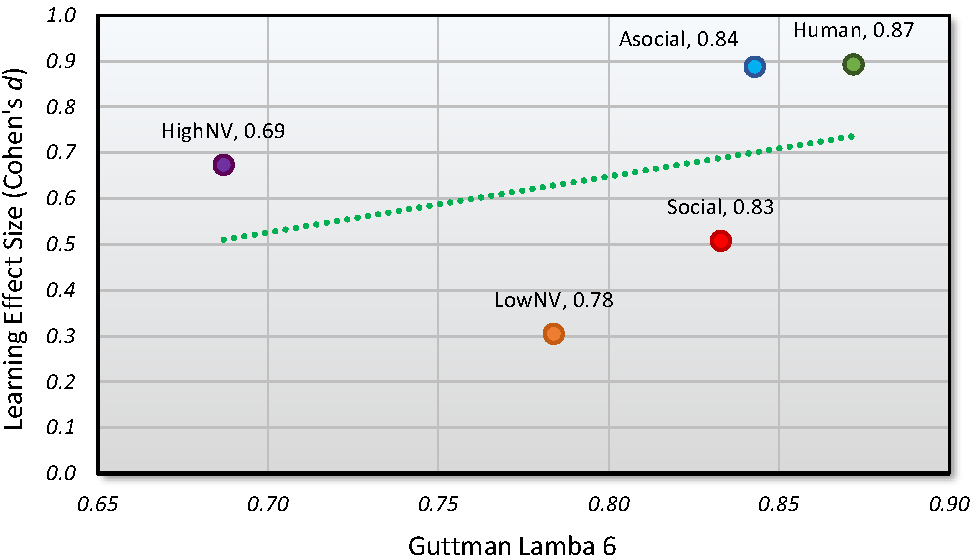
\includegraphics[width=0.75\textwidth]{images/ch10_guttmang6.pdf}
    \caption{Guttman's Lambda 6 against \gls{learning} effect size for each of the prime tutoring conditions. The dotted line indicates a trend towards greater internal consistency (measured through G6) leading to greater \gls{learning}.}
    \label{fig:ch10-guttmangraph}
\end{figure}

\paragraph{A Proposed Model}
Taking Guttman's Lambda 6 to provide a reasonable indication of the congruency of social cues, then it is clear that this alone would not provide a strong predictor of \gls{learning} (Figure \ref{fig:ch10-guttmangraph}). However, this data can be combined with the social behaviour (as measured through \acrshort{nvi}) to be compared to \gls{learning} outcomes. In the resulting space, both congruency and social behaviour could have an impact on \gls{learning}, as hypothesised in the previous section (Figure \ref{fig:ch10-3dgraph}).

\begin{figure}[t]
    \centering
    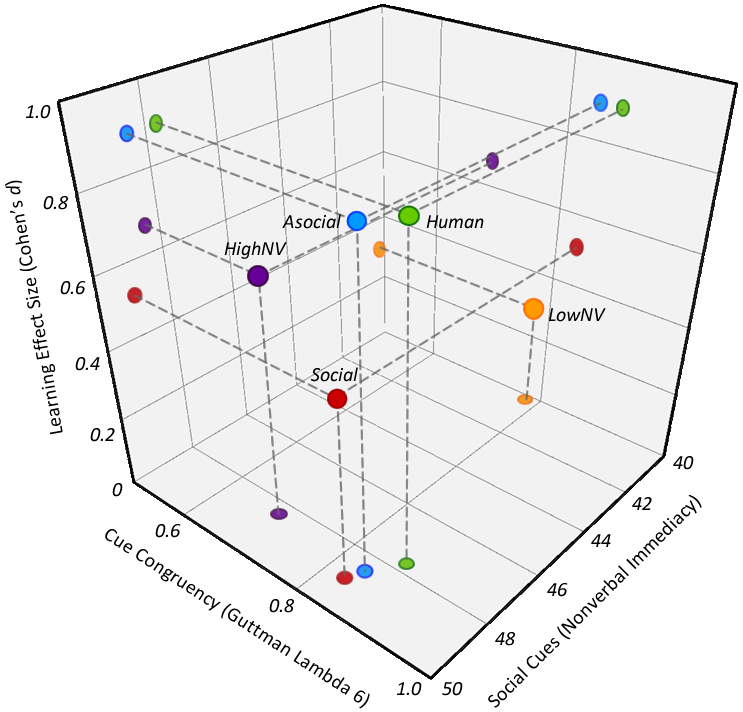
\includegraphics[width=0.75\textwidth]{images/ch10_3dplot.png}
    \caption{Learning, congruency and social behaviour for each of the 5 conditions. Learning is measured in effect size between pre- and post-test for children. Congruency is indicated through Guttman's Lambda 6 of the adult \gls{nonverbalimm} scores. Social behaviour is characterised through \gls{nonverbalimm} ratings from adults. An interactive version of this figure is available online to provide different perspectives of the space: \url{https://goo.gl/ZNPxc8}.}
    \label{fig:ch10-3dgraph}
\end{figure}

The data shows that \gls{learning} is best with human behaviour which is shown to be highly social and congruent. When the social behaviour used is congruent, but not highly social, then the \gls{learning} drops to a low level. With roughly congruent social behaviour as characterised by \gls{nonverbalimm} (social, asocial, and human conditions), when the congruency of the cues increases (indicated by Guttman's G6), \gls{learning} also increases. The combination of congruency and social behaviour as characterised by \gls{nonverbalimm} appears to provide a reasonable model for \gls{learning} predictions, where the combination of high social behaviour and social cue congruency is necessary to maximise potential \gls{learning}.

Such a model is supported by the view of social cues being perceived as a single percept, as suggested by \cite{zaki2013cue}. Experimental evidence with perception of emotions would seem to provide additional weight to such a perspective \citep{nook2015new}. This has clear implications for designers of social robot behaviour when human perceptions or outcomes are of any degree of importance. The combination of all social cues in context must be considered alongside the expectations of the human in order to generate appropriate behaviour. Not only does this give rise to a number of challenges, such as identifying combinatorial contextual expectations for social cues, but it could also have implications for how social cues should be examined experimentally. The isolation of specific social cues in experimental scenarios would not describe the role of that social cue, but the role of that social cue, \textit{given the context of all other cues}. This is an important distinction that leads to a great deal more complexity in `solving' behavioural design for social robots, but that would also contribute to explanations of why a complex picture is emerging in terms of the effect of robot behaviour on \gls{learning}, as discussed in Chapter \ref{chap:background}.

This model lends itself to generating predictions concerning social behaviour, social cues and \gls{learning}, as well as providing retrospective characterisation of social behaviour. The following predictions can be derived from the extremities of the space that is presented:
\begin{enumerate}
	\item [P1.] Highly social behaviour of a tutor robot (as characterised by \gls{nonverbalimm}) with high congruency will lead to maximum potential \gls{learning}.
	\item [P2.] Low social behaviour of a tutor robot with low congruency will lead to minimal potential \gls{learning}.
	\item [P3.] A mismatch in the social behaviour of a tutor robot and the social cue congruency will lead to less than maximum potential \gls{learning}.
\end{enumerate}

An accurate, or reliable measure for social cue congruency would be desirable in order to properly measure or characterise the social cue congruency dimension (rather than the indicator used here). However, this would not necessarily be something that would be straightforward to achieve due to the potentially complex interactions between large numbers of social cues. Additionally, the data used for the learning axis was collected with relatively few samples (just over 10 per condition) in a specific experimental setup. Ideally, many further samples would be collected in both the short and long-term. The data collected here is over the short term and with children unfamiliar with robots. As longer-term interactions take place, or as robots become more commonplace in society, expectations may change and the model will need revision to account for this. Nevertheless, these predictions support the thesis contained in this document: `a robot with \gls{tailored} social behaviour will positively influence the outcomes of tutoring interactions with children and consequently lead to an increase in child \gls{learning} when compared to a robot without this social behaviour'.

%%%%%%%%%%%%%%%%%%%%%%%%%%%%%%%%%%%%%%%%%%%%%%%%%%%%%%%%%%%%%%%%%%%%%%%%%%%%%%
\section{Summary} \label{sec:behave-summary}
This chapter brought together the findings from the previous chapters in the context of the thesis for this work: that tailored social behaviour of a robot will lead to better child \gls{learning}. An additional experimental condition was introduced to provide a benchmark and further context for the child \gls{learning}, and behavioural ratings of the robot conditions. Nonverbal immediacy was used to tie the findings together in support of the thesis. The relationship between child \gls{learning} and robot social behaviour was then discussed in a broader context, drawing on other literature as well as the data from the work conducted here. A model of the relationship between social behaviour and \gls{learning} was proposed, with the intention of providing a working hypothesis for future research. Robot social cues and the congruency between the cues are suggested to have a combined effect on \gls{learning}.